% As this work, aims to compare techniques of word similarity based on two approaches,  lexical bases and distributional, we did some evaluation on 
% use a common portuguese dataset for evaluation called PT65 and 
% In order to be able to generate the word embeddings using multiple algorithms, it is required a corpus. For this, we got a portuguese Wikipedia dump and did some pre-processing to generate a corpus suitable for the given task.
% This work aims to compare techniques based on lexical bases with the distributional based ones.

% - Explore the existing techniques regarding word similarity, using a distributional approach called word embeddings, adapting existing works to Brazilian Portuguese.
% - Compare the word embeddings approach to other techniques that are solely based on a lexical database such as WordNet.
% - Adapt existing studies regarding the addition of syntactic context in the training process of word embeddings to a Brazilian Portuguese corpus, to check if the results will be, similar or not. 
% - Evaluate the different techniques over a common \textit{dataset}.

% \subsubsection{WordSimilarity-353 Test Collection}
% The WordSimilarity-353 is a test collection for measuring word similarity developed by \citetexto{Finkelstein:2001:PSC:371920.372094}. This dataset contains two sets of English word pairs along with human-assigned similarity judgements.
% http://www.cs.technion.ac.il/~gabr/resources/data/wordsim353/
% \subsubsection{ENSEPRO Word Similarity}
% Aiming to prove an improvement in the accuracy of information extraction systems, a specific dataset will be assembled using the questions and answers of short sentences used in the ENSEPRO system. This system evaluation was made using the dataset for the challenge Question Answering over Linked Data (QALD-7) of 2017, which also had the addition of the Portuguese language. For each sentence of the Portuguese questions of this dataset, we will assemble a new dataset with only the keywords necessary to carry out queries via the ENSEPRO search engine. A pair of this keyword must be generated with the one that is currently in the linked data. For words that the system currently cannot find answers due to lack of a word in the expansion of related terms, it will be investigated manually which would be the word that should be found and added to the dataset. Also, the dataset will include the syntactic information for each keyword.



\section{Methods and materials}\label{chap:methodsandmaterials}

This chapter will present a description of what and how this work was done, as well as the tools and methods used. First ~\autoref{chap:methodsandmaterials:architecture} presents an overview of the architecture and how the proposed experiment was realized. Then, the ~\autoref{chap:methodsandmaterials:dataset} presents the dataset used in the evaluation process. After that we start with a detailed explanation of the Corpus generation in ~\autoref{chap:methodsandmaterials:corpus}, of the syntactic parsing in ~\autoref{chap:methodsandmaterials:palavras}. Then we explain how we generate the most common word embedding models in ~\autoref{chap:methodsandmaterials:wegeneration} and at last we explain how we reproduced the work of \citetexto{Levy2014} for Portuguese in ~\autoref{chap:methodsandmaterials:depsgeneration}.

\subsection{Architecture overview}\label{chap:methodsandmaterials:architecture}

The proposed work consists of comparing different word similarity techniques. Therefore, ~\autoref{fig:arq} defines an overview of the architecture with the intention of comparing several techniques using different algorithms and testing them with a common dataset.

\begin{figure}[h]
    \caption{Proposed architecture}
    \label{fig:arq}
    \centering%
    \begin{minipage}{.8\textwidth}
        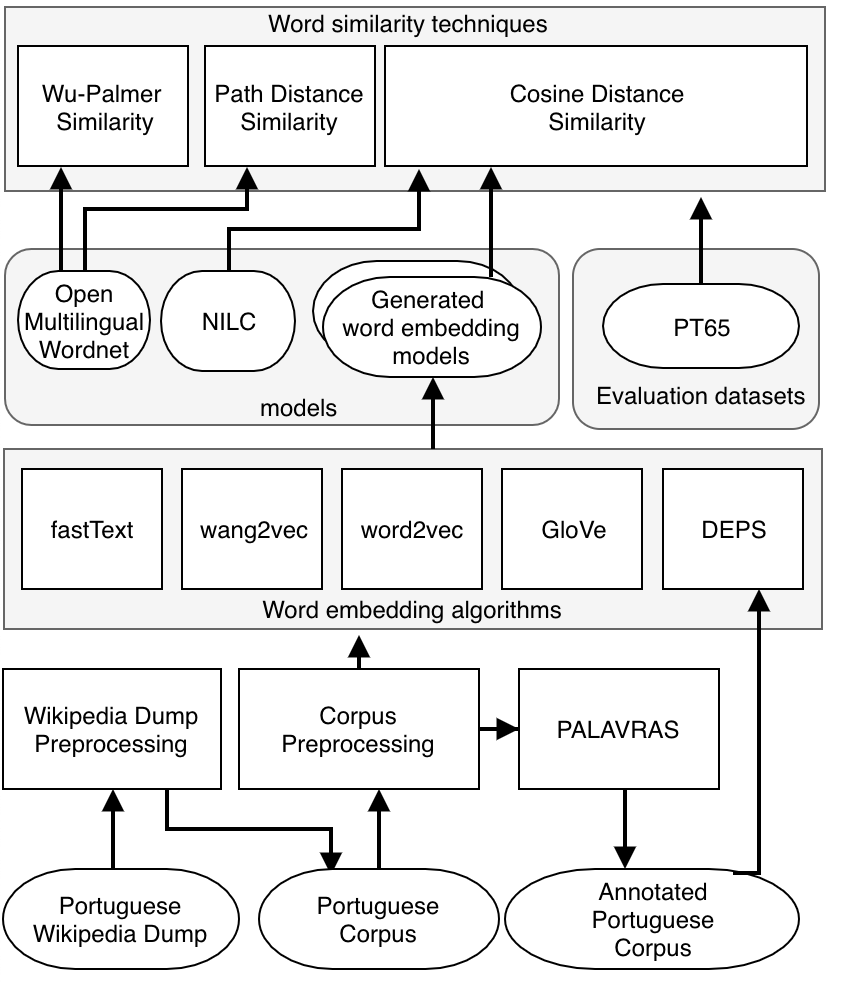
\includegraphics[width=\textwidth]{arq.png}
        \fonte{Made by the author.}
    \end{minipage}
\end{figure}


In this work, we compared techniques based on the two main approaches to word similarity, the knowledge-based and the distributional-based. 

Regarding the knowledge-based approach we utilized a lexical base, in this case, \textbf{Open Multilingual Wordnet} (OMW) wore used with \textbf{Path Distance} and \textbf{Wu-Palmer} similarity techniques. It was decided to use OMW due to its ease of use through the \textbf{Natural Language Toolkit} (NLTK) library available for the \textbf{Python version 3.6} programming language as well as the availability of the Portuguese language for querying the synsets. \cite{Bond2013LinkingAE}.

For the distributional approach we \textbf{generated word embedding models} with a corpus obtained from the \textbf{Brazilian Portuguese Wikipedia dump} of articles. The word embeddings wore generated using several different model implementations for learning word representations. In this case, \textbf{FastText}, \textbf{Wang2vec}, \textbf{Word2vec} and \textbf{GloVe}. Also, we compare our word embedding models with a set of pre-trained models available from \textbf{Núcleo Interinstitucional de Linguística Computacional} (NILC) in all different implementations (FastText, Wang2vec, Word2vec, and GloVe). One thing to note is that the metric used for the comparison of similarity between one word and another for all word embedding models was the \textbf{cosine distance}. The \textbf{CBOW} and \textbf{Skip-gram} were used for the models that has this option. \cite{bojanowski2016enriching,Ling:2015:naacl,Mikolov2013DistributedRO,Pennington2014,Hartmann2017}

We also generated one more model in order to take into account the syntactic tree information of the sentences from the Portuguese corpus using the algorithm implementation by \citetext{Levy2014} which generates the \textbf{DEPS} model. In order to do this, we used the \textbf{PALAVRAS syntactic parser} to annotate the corpus with syntactic information. \cite{bick2000palavras}.

In the end, we do a quantitative evaluation of all models and techniques using the \textbf{PT65} dataset, which consists of a pair of words and a similarity value given by persons. \cite{GranadaSV14}.

All the experiments were done using the \textit{Semantics} computer (Intel(R) Xeon(R) CPU E5-2620 v4 @ 2.10GHz with 32 cores and 128GB of RAM) granted by the \textit{UNISINOS Programa de Pós-graduação em Computação Aplicada} (PPGCA) by running \textbf{Docker} containers.


\subsection{PT65 Dataset}\label{chap:methodsandmaterials:dataset}

This dataset is composed of 65 word pairs, initially generated by \citetexto{Rubenstein1965ContextualCO} on the name of \textit{RG65}. This word pairs wore translated to Portuguese by \citetexto{GranadaSV14} and evaluated with 50 persons. 

The initial idea was to use the WordSimilarity-353 Test Collection developed by \citetexto{Finkelstein:2001:PSC:371920.372094} which consists of two sets of English word pairs along with human-assigned similarity judgments. However, we would have to translate to Portuguese and then the human-assigned similarity judgments would not fit entirely regarding the semantic changes involved in the translation process. So the PT65 dataset was used in the evaluation process.

\subsection{Corpus generation}\label{chap:methodsandmaterials:corpus}

In this section, I will present the process involved in generating a corpus that can be used on NLP tasks from a Wikipedia dump. I’ve used this process to generate the Word Embeddings for evaluation in this thesis. While I focus on the Portuguese language, you could easily do the same thing for the other available languages in Wikipedia.

\subsubsection{Getting the Wikipedia PT-BR dump}

First, we downloaded the latest Portuguese Wikipedia articles dump\footnote{\url{https://dumps.wikimedia.org/ptwiki/latest/ptwiki-latest-pages-articles-multistream.xml.bz2}}. The file is a big, compressed XML file that contains all articles in the wiki text format, just like markdown but with some special tokens that deal with some specific Wikipedia features. For example: "\textit{[[Imagem:Starsinthesky.jpg|thumb|[[Estrela|Formação estrelar]] na [[Grande Nuvem de Magalhães]], uma [[galáxia irregular]].]]}"

% \begin{lstlisting}
%     @[[Imagem:Starsinthesky.jpg|thumb|[[Estrela|Formação estrelar]] na [[Grande Nuvem de Magalhães]], uma [[galáxia irregular]].]]@
% \end{lstlisting}

You can find more detailed information about the dump formats and different languages in their website\footnote{\url{https://en.wikipedia.org/wiki/Wikipedia:Database_download}}.

\subsubsection{Preprocessing with Wikiextractor}

As described in the previous step, the format of the dump is not suitable for most of NLP tasks. That’s why we need to parse the wiki text format to raw text. In order to do this, we have a few options. We could use the python \textbf{gensim.corpora.WikiCorpus} class but its tokenizer is not so good for Portuguese (In our case we need to have words separated by ‘-’ like ‘guarda-chuva’ which is very common in Portuguese). So, we ended up using the \textbf{wikiextractor} project that just reads the XML file and outputs all the documents in parsed text. We chose to cleanup and tokenize the corpus in a later stage. So, we just cloned the repository and executed the \textbf{wikiextractor}.

% \begin{lstlisting}[language=sh]
% git clone https://github.com/attardi/wikiextractor.git
% cd ./wikiextractor
% python ./WikiExtractor.py --no-templates -o ../data/ptwiki-articles-text/ -b 10M -c ../data/ptwiki-latest-pages-articles-multistream.xml.bz2
% cd ..
% \end{lstlisting}

Wikipedia has a concept of Templates, which consists of using other documents inside of a given one. For the objective of this corpus, it is not desired that the tool expands these templates, because it will just add duplicated sentences to the content. So, it is really important to use the \textit{–no-templates} flag.
This tool generated multiple compressed 10MB files of wiki articles sentences as seen in ~\autoref{fig:wikiextractor}.

\begin{figure}[h]
	\caption{WikiExtractor output sample.}
	\label{fig:wikiextractor}
	\centering%
	\begin{minipage}{.9\textwidth}
		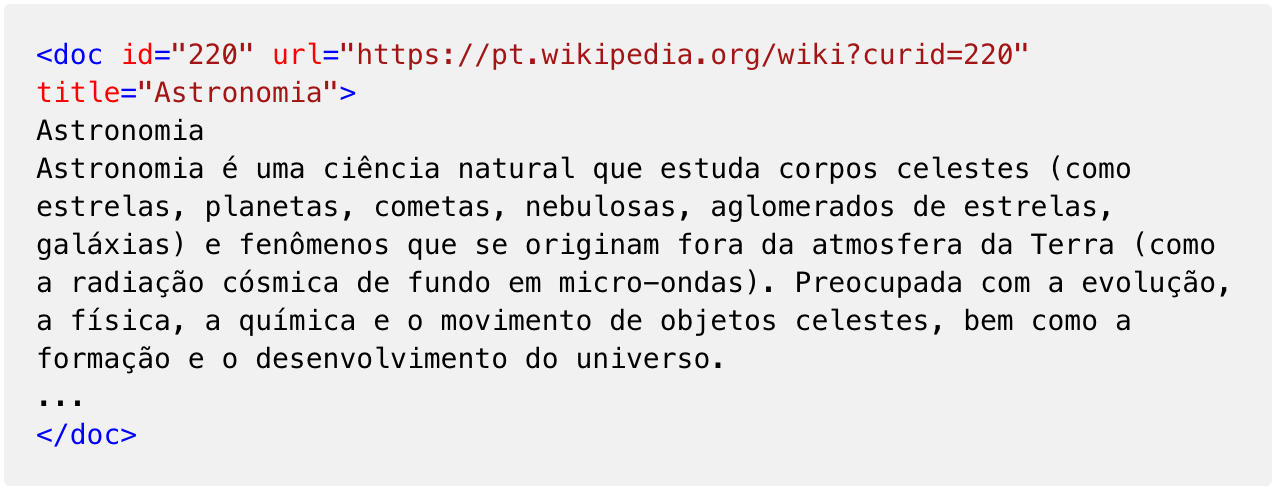
\includegraphics[width=\textwidth]{wikiextractor.png}
		\fonte{Made by the author.}
	\end{minipage}
\end{figure}



% \begin{lstlisting}[language=XML]
% <doc id="220" url="https://pt.wikipedia.org/wiki?curid=220" title="Astronomia">
% Astronomia 
% @Astronomia é uma ciência natural que estuda corpos celestes (como estrelas, planetas, cometas, nebulosas, aglomerados de estrelas, galáxias) e fenômenos que se originam fora da atmosfera da Terra (como a radiação cósmica de fundo em micro-ondas). Preocupada com a evolução, a física, a química e o movimento de objetos celestes, bem como a formação e o desenvolvimento do universo.@
% ...
% </doc>
% \end{lstlisting}

It is also possible to save this as only one text file just by changing the tool arguments.
At the time of writing, there were 1,000,400 documents in the ptwiki-dump.

\subsubsection{Custom preprocessing}

In order to cleanup the sentences for generating the Word embedding models we did some custom pre-processing\footnote{\url{https://github.com/eberlitz/pt-br-word-embeddings/blob/master/scripts/preprocess.py}} based on \citetexto{Hartmann2017} preprocessing scripts. Some changes were made to do the some cleaning as follows:

\begin{itemize}
    \item Breaks an entire document into multiple sentences using the 
    \textbf{nltk.data.load ('tokenizers/punkt/portuguese.pickle')}. (Natural Language Toolkit - NLTK is a leading platform for building Python programs to work with human language data, and it has a sentence segmentation tool called \textbf{punkt}.)
    \item Does not change the current letter case. (Later I'll use a Syntactic parser that has better accuracy if I maintain this)
    \item Remove sentences with less than 4 tokens (as it does not add meaningful value to the corpus we can remove very short sentences).
    \item Allow abbreviations, like 'Dr.'.
    \item Keep words with '-', like 'guarda-chuva' (which means umbrella in English).
    \item All emails are mapped to EMAIL token.
    \item All numbers are mapped to 0 token.
    \item All URLs are mapped to URL token.
    \item Different quotes are standardized.
    \item Different kinds of hyphenation are standardized.
    \item HTML strings are removed.
    \item All text between brackets is removed.
\end{itemize}

With this, we ended up with the final 1.6GB PT-BR corpus file which contains 9.896.520 sentences, 251.193.592 tokens and 3.137.040 unique tokens.

% --------------------------------------------------------

\subsection{PALAVRAS annotated corpus generation}\label{chap:methodsandmaterials:palavras}

To annotate all sentences of the corpus with syntactic tags, we used the software PALAVRAS developed by \citetexto{bick2000palavras}, which is an automatic parser for Portuguese.

First, we tried to use the parser with multiple sentence files of 1MB. However, the parser was taking too much time to execute and sometimes errors occurred. So we wrote a Python script that sends sentences in batches to the PALAVRAS parser and saves the results. Also, we have used parallel computing doing this process times the number of cores on the machine. Although, we first run this on a i5 2.4GHz computer with 4 cores, achieving an average speed of 16 sentences per second, which means that for all 9896520 sentences it would take 7 days to complete. We have tried other techniques attempting to increase the speed, but the bottleneck was indeed in the parser tool. 

With this problem at hand, \textit{UNISINOS Programa de Pós-graduação em Computação Aplicada} (PPGCA) granted us access to the \textit{Semantics} computer (Intel(R) Xeon(R) CPU E5-2620 v4 @ 2.10GHz with 32 cores and 128GB of RAM). With 32 cores the parsing step should be concluded in 24 hours.

One more problem that we had is that the PALAVRAS could not parse some of the sentences. Since we were running the parser in batches, this means that if one sentence failed, we lost all the parsed sentences in the batch. Also, as this process would take too long, we had to implement some way to continue the process if some fatal error occurred. With this in mind, we converted the sentences file to an SQLite table with three columns (id, text and parsed text). With this whenever we start the parsing process, we can continue from where it stopped.

With this solution implemented, we created a docker image and started running in the Semantics machine. The overall process took 38 hours. 24 hours to process 8916000 sentences using batches of 30, and 14 hours to process the remaining ones without sending in batches. Resulting in a 15GB corpus file.

% --------------------------------------------------------

\subsection{Common Word Embeddings generation}\label{chap:methodsandmaterials:wegeneration}

In order to have a base for comparison, we generated all models that were used by \citetexto{Hartmann2017}. In this case, FastText, Wang2vec, Word2vec and GloVe using different dimensions values as 50, 100, 300, 600 and 1000. \cite{bojanowski2016enriching, Ling:2015:naacl, Mikolov2013DistributedRO, Pennington2014}. Also the CBOW and Skip-gram were used for the models that has this option.

For this, we downloaded all those model generation tools from GitHub, compiled into a docker image, and use as input our corpus text file. We only created some script to run this several times with different dimension sizes as it took several hours to complete.

% --------------------------------------------------------

\subsection{DEPS Word Embedding generation}\label{chap:methodsandmaterials:depsgeneration}

In order to generate the DEPS (dependency-based syntactic contexts) word embedding model proposed by \citetexto{Levy2014}, we got the source code called \textit{word2vecf} from their website. The input required by this model is three files, a word and context vocabulary, and a contexts file. 

The vocabulary files are just a list of words or contexts with the total number of occurrences. The contexts file is a multiline context per word, where one word can have multiple contexts. In the form of "<\textit{word}> <\textit{dependency-relation}>\_<\textit{referred-word}>".

In order to generate this file from our corpus we got the annotated output from the PALAVRAS parser and extracted the syntactic tags. This process is shown by in ~\autoref{fig:deps-context}.

\begin{figure}[h]
	\caption{DEPS contexts generation from parsed sentence. Left: Sample output from the PALAVRAS parser for the sentence "A astronomia é uma das mais antigas ciências.". Right: Sample of our generated contexts file for an annotated sentence.}
	\label{fig:deps-context}
	\centering%
	\begin{minipage}{.95\textwidth}
		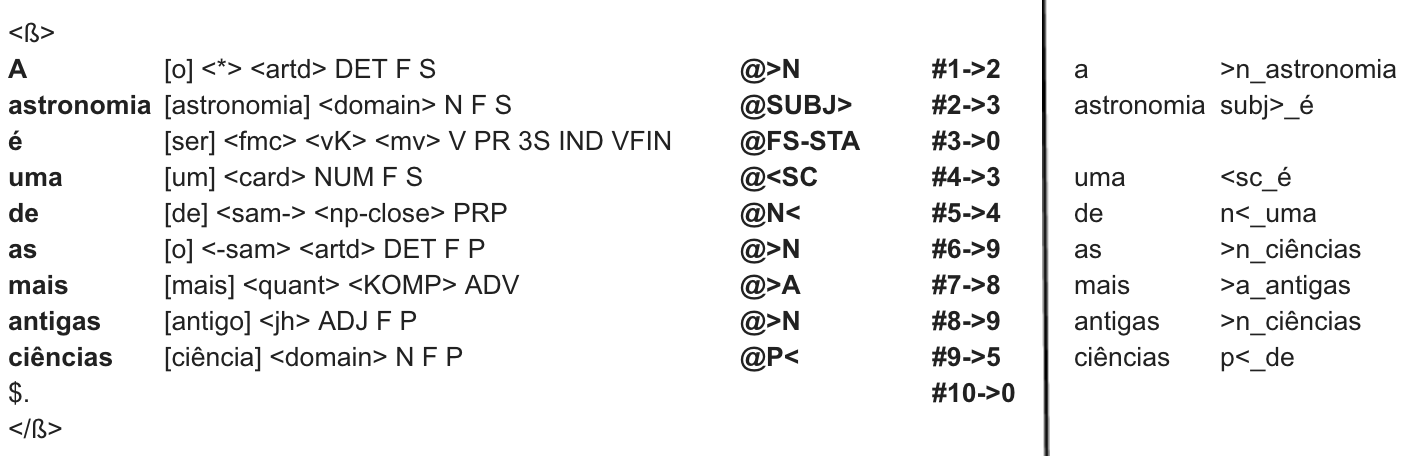
\includegraphics[width=\textwidth]{deps-context.png}
		\fonte{Made by the author.}
	\end{minipage}
\end{figure}

The generation of this three files was not trivial and the implemented code to do so had to use a map-reduce approach in order to use all computation resources available. It took 14 hours to process all 9896000 parsed sentences with an average speed of 196.2 sentences per second.

After we had the input files, we just run the \textit{word2vecf} tool which took some hours to complete. We generated models with different dimensions values as 50, 100, 300, 600 and 1000.








% CÓDIGO: https://levyomer.wordpress.com/2014/04/25/dependency-based-word-embeddings/
% DATASET: http://www.cs.technion.ac.il/~gabr/resources/data/wordsim353/

% resources:
% - Open Multilingual Wordnet
% - NILC Pre-trained word embeddings models
% Corpus:
%  - Pegar com o allan o corpus portugues
%  - Anotar o corpus com o PALAVRAS syntactic parser
% quantitative evaluation datasets:
%  - WordSim353 manual translation to portuguese
%  - ENSEPRO word similarity (vou criar em conjunto com o denis, preciso definir formato e como, usando as perguntas do QALD)
% Algoritmo:
%  - Usar o código fonte do DEPS
% tools:
%  - Palavras
%  - Python NLTK, word2vec, word2vecf, 













% \begin{itemize}
%     \item Explore the existing techniques regarding word similarity, using a distributional approach called word embeddings, adapting existing works to Brazilian Portuguese.
%     \item Compare the word embeddings approach to other techniques that are solely based on a lexical database such as WordNet.
%     \item Adapt existing studies regarding the addition of syntactic context in the training process of word embeddings to a Brazilian Portuguese corpus, to check if the results will be, similar or not. 
%     \item Evaluate the different techniques over a common \textit{dataset} related to \citetexto{denis2018} work.
% \end{itemize}

% This thesis is structured as follows. The \autoref{chap:background} presents the general concepts and techniques used in this work. In \autoref{chap:relatedwork} are described and analyzed the works related to the research area of this work. The \autoref{chap:methodsandmaterials} presents the proposed model, as well as the form of the experiment and the necessary tools. The \autoref{chap:results} presents the preliminary results obtained in the case study experiment. Finally, \autoref{chap:conclusions} summarizes the thesis findings, contributions, and discusses.





% Descrever um cenário em que o projeto se faz necessário (Extração de informação em ontologias utilizando Linguagem Natural - Talvez citar o uso de queries que utilizem triplas RDF) e ajuda a resolver o problema. Após descrito citar como exemplo o trabalho do denis e detalhar o cenário dele.

% - Cenário do denis: Recebe uma pergunta; Realiza um parse, extraindo palavras relevantes e seu contexto sintático; Realiza a geração de combinações diferentes de possíveis tuplas RDF de pesquisa; Algumas dessas pesquisas não se encontra a resposta, porém se uma destes elementos da tupla fosse substituído por um outro sinônimo ele iria encontrar a resposta. Portanto é usado o WordNet BR para procurar por sinônimos, porém ainda assim, nem sempre se tem a palavra cadastrada no WordNet.

% Descrever a arquitetura do modelo proposto.

% - Usar o NLTK python e procurar por sinônimos de uma dada palavra no OpenWordNet-PT ( supõe-se que algumas vezes não será encontrado nada )
% - Usar diferentes tipos de word embedding (BoW, SG, GloVe)
% - [TCC2]Treinar word embeddings sobre um corpus (pegar com o allan) utilizando o contexto gerado pelo POS Tagger da unisinos (Aonde consigo??)
% - [TCC2]Algum outro algoritmo se houver necessidade
% - Testar cada abordagem com o dataset do denis




% OpenWordNet-PT. \cite{coling2012}.

